\section{Mérési adatok}

Az elkészült szoftverrel analizáltam 11000 Twitter felhasználó tweetjeit,
közben figyelemmel kísértem a szoftver teljesítményét.

Az adatbázis a futás során másodpercenként 20 kérést szolgált ki,
ez túlnyomórészt írási művelet (\ref{fig:req-per-sec}. ábra).

Az adatbázis válaszideje meglepően magas volt, hét párhuzamosan futó worker
folyamat mellett 200ms körüli értékeket mutatott, ez feltehetően a sor
járulékos műveletre vezethető vissza (számláló inkrementálás).
A válaszidőket \aref{fig:mean-db-time}. ábra mutatja.

\begin{figure}[h!]
  \centering
  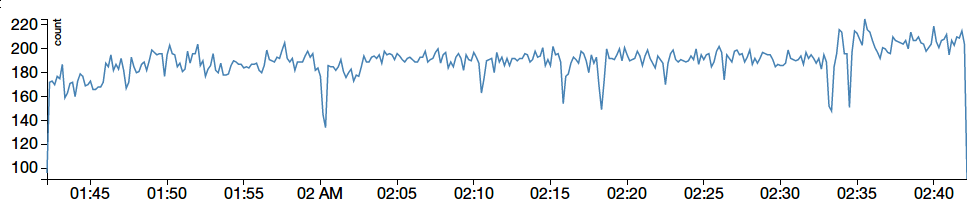
\includegraphics[width=0.9\textwidth]{figures/req-per-sec}
  \caption{Adatbázis kérések száma 10 másodperces időablakokban}
  \label{fig:req-per-sec}
\end{figure}

\begin{figure}[h!]
  \centering
  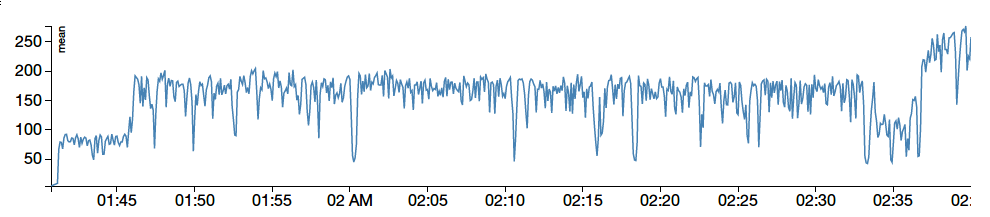
\includegraphics[width=0.9\textwidth]{figures/mean-db-time}
  \caption{Átlagos adatbázis válaszidő 7 worker folyamat mellett (ms)}
  \label{fig:mean-db-time}
\end{figure}

\Aref{fig:queue-progress}. ábrán az üzenetsor állapota látható a
\emph{fetch-followers} futása során. Ekkor kerülnek beütemezésre az egyes
felhasználók tweetjeit lekérdező jobok \emph{fetch-tweets}.

\begin{figure}[h!]
  \centering
  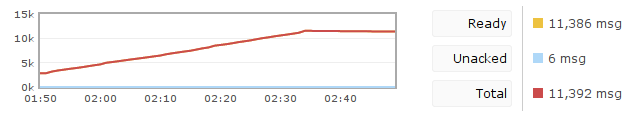
\includegraphics[width=0.6\textwidth]{figures/queue-progress}
  \caption{A fetch-tweets feladatok felhalmozódása}
  \label{fig:queue-progress}
\end{figure}

Az egyes worker folyamatok teljesítményét szintén nyomon tudtam
követni.
\Aref{fig:mean-twitter}. ábrán a Twitter API átlagos válaszideje,
\aref{fig:mean-worker}. ábrán pedig az egyes jobok átfutási ideje látható.
Leolvasható, hogy a külső szolgáltatás viszonylag gyors,
a szűk keresztmetszetet az adatbázis jelenti.

\begin{figure}[h!]
  \centering
  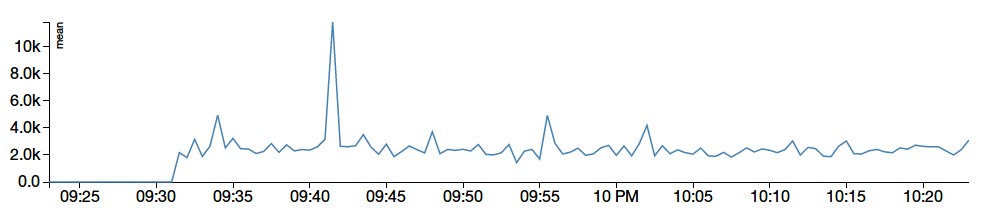
\includegraphics[width=0.9\textwidth]{figures/mean-twitter}
  \caption{A Twitter API átlagos válaszideje (ms)}
  \label{fig:mean-twitter}
\end{figure}

\begin{figure}[h!]
  \centering
  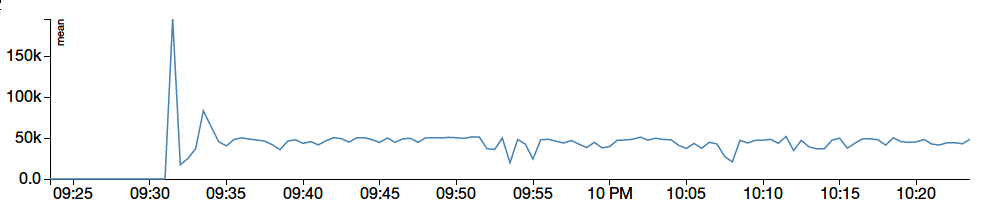
\includegraphics[width=0.9\textwidth]{figures/mean-worker}
  \caption{A jobok átlagos feldolgozási ideje (ms)}
  \label{fig:mean-worker}
\end{figure}

Az adatbázis sebessége az aggregációs fázisban nagyságrendekkel jobb,
átlagosan 15ms (\ref{fig:mean-read}. ábra). A folyamat során több mint
egy millió tweet került feldolgozásra.

\begin{figure}[h!]
  \centering
  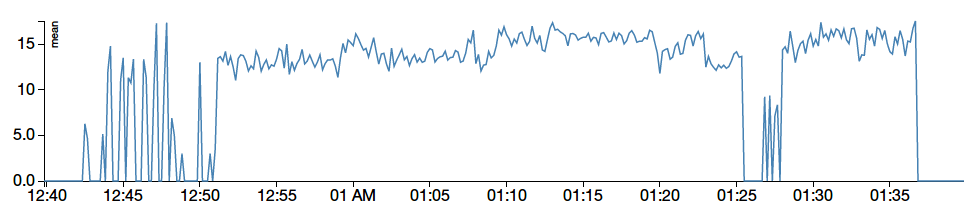
\includegraphics[width=0.9\textwidth]{figures/mean-read}
  \caption{Átlagos válaszidő olvasás esetén (ms)}
  \label{fig:mean-read}
\end{figure}
